% This file was created with tikzplotlib v0.10.1.
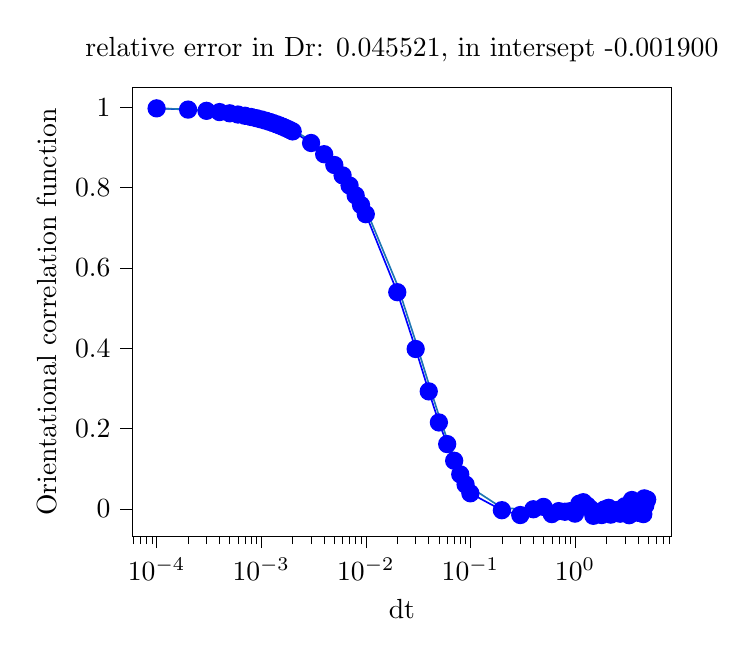
\begin{tikzpicture}

\definecolor{darkgray176}{RGB}{176,176,176}
\definecolor{steelblue31119180}{RGB}{31,119,180}

\begin{axis}[
log basis x={10},
tick align=outside,
tick pos=left,
title={relative error in Dr: 0.045521, in intersept -0.001900},
x grid style={darkgray176},
xlabel={dt},
xmin=5.8276061909058e-05, xmax=8.40825519000689,
xmode=log,
xtick style={color=black},
y grid style={darkgray176},
ylabel={Orientational correlation function},
ymin=-0.067477524201761, ymax=1.04778267118092,
ytick style={color=black}
]
\addplot [semithick, blue, mark=*, mark size=3, mark options={solid}]
table {%
0.0001 0.996869693545151
0.0002 0.993750595175417
0.0003 0.990648067986856
0.0004 0.987559120179852
0.0005 0.984484804565174
0.0006 0.981424405000625
0.0007 0.978373415925522
0.0008 0.975331233041958
0.0009 0.972301613836295
0.001 0.969284244964802
0.0011 0.966270397132604
0.0012 0.963267704178855
0.0013 0.960273485471981
0.0014 0.957279600974771
0.0015 0.954294750346964
0.0016 0.951316772974624
0.0017 0.948348638896533
0.0018 0.945391246032783
0.0019 0.942444880056686
0.002 0.939505588675522
0.003 0.910618621274521
0.004 0.882786995930552
0.005 0.855984560312999
0.006 0.830090716897695
0.007 0.804783134950062
0.008 0.780215354996437
0.009 0.756510218433539
0.01 0.733608597868951
0.02 0.539512636985611
0.03 0.398183942634591
0.04 0.292817678536257
0.05 0.215491967276188
0.06 0.161659961969084
0.07 0.120236813652894
0.08 0.086454302477147
0.09 0.0609180847676956
0.1 0.0392763923453193
0.2 -0.00282482229585721
0.3 -0.0148360605970167
0.4 -0.000489055092350786
0.5 0.00534602877754716
0.6 -0.0125123931031099
0.7 -0.00507160411676968
0.8 -0.00663074746480157
0.9 -0.0050695586339019
1 -0.0113321122049239
1.1 0.0132949749647517
1.2 0.017049492205019
1.3 0.00913424619466558
1.4 0.000927730467969487
1.5 -0.0167838789570939
1.6 -0.00981594409218044
1.7 -0.00745025920879516
1.8 -0.0148531907332659
1.9 -0.00135551050561091
2 0.000386129799057489
2.1 0.00307850208718348
2.2 -0.013817047621389
2.3 -0.00283744677311522
2.4 -0.00792766216376173
2.5 -0.00751774768459356
2.6 -0.00175442753027467
2.7 -0.01149170267198
2.8 -0.00493744910855688
2.9 -0.0006640652652671
3 0.00705980472571085
3.1 -0.00413643487740399
3.2 0.00268026972386226
3.3 -0.0152625491893496
3.4 0.00966372359702825
3.5 0.02252743351477
3.6 -0.00842334747212407
3.7 0.00196390149066854
3.8 -0.00193245255738091
3.9 -0.00656658319262955
4 -0.00914694318526369
4.1 0.00856952775668696
4.2 0.00203322496745534
4.3 0.00540117085980926
4.4 -0.00635525274573206
4.5 -0.0125112297957198
4.6 0.0265895508806756
4.7 0.00892382779312096
4.8 0.0203085013691107
4.9 0.0236685940651422
};
\addplot [semithick, steelblue31119180]
table {%
0.0001 0.997089025936249
0.0002 0.994186525642498
0.0003 0.991292474451822
0.0004 0.988406847769101
0.0005 0.985529621070811
0.0006 0.982660769904815
0.0007 0.979800269890157
0.0008 0.97694809671685
0.0009 0.974104226145677
0.001 0.971268634007976
0.0011 0.968441296205444
0.0012 0.965622188709925
0.0013 0.962811287563207
0.0014 0.960008568876824
0.0015 0.957214008831845
0.0016 0.954427583678676
0.0017 0.951649269736859
0.0018 0.948879043394868
0.0019 0.946116881109908
0.002 0.94336275940772
0.003 0.916258658703931
0.004 0.889933295837348
0.005 0.864364296606157
0.006 0.839529929649928
0.007 0.815409087979898
0.008 0.791981271039925
0.009 0.769226567282849
0.01 0.747125637247457
0.02 0.558196717832419
0.03 0.417043078519985
0.04 0.311583575798885
0.05 0.232792077624583
0.06 0.173924929341426
0.07 0.129943773667432
0.08 0.0970843247076193
0.09 0.0725341879639191
0.1 0.0541921514047699
0.2 0.0029367892738775
0.3 0.000159150928973874
0.4 8.62473123916195e-06
0.5 4.67392741138113e-07
0.6 2.53290181932471e-08
0.7 1.37263398886261e-09
0.8 7.4385988947776e-11
0.9 4.03113677545142e-12
1 2.18455974468599e-13
1.1 1.18385992436788e-14
1.2 6.41559162633841e-16
1.3 3.47674712765705e-17
1.4 1.88412406738089e-18
1.5 1.02104736724876e-19
1.6 5.53327535173865e-21
1.7 2.99860095625702e-22
1.8 1.62500637023969e-23
1.9 8.80625912497442e-25
2 4.77230127810253e-26
2.1 2.58621273412109e-27
2.2 1.40152432052433e-28
2.3 7.59516181753216e-30
2.4 4.11598159159435e-31
2.5 2.23053897590927e-32
2.6 1.20877705896715e-33
2.7 6.55062293941603e-35
2.8 3.54992350128392e-36
2.9 1.92377991856926e-37
3 1.04253772616563e-38
3.1 5.64973623015521e-40
3.2 3.06171361181585e-41
3.3 1.65920847609569e-42
3.4 8.99160769486551e-44
3.5 4.87274565572452e-45
3.6 2.64064570331958e-46
3.7 1.43102271760647e-47
3.8 7.75501997761952e-49
3.9 4.20261216774172e-50
4 2.2774859488979e-51
4.1 1.23421863364909e-52
4.2 6.68849630613008e-54
4.3 3.6246400449205e-55
4.4 1.96427042102118e-56
4.5 1.06448040055892e-57
4.6 5.76864830344984e-59
4.7 3.12615462261427e-60
4.8 1.69413044623436e-61
4.9 9.18085736417613e-63
};
\end{axis}

\end{tikzpicture}
